%        File: pokemon.tex
%     Created: Sun Jan 07 22:00 PM 2012 C
% Last Change: Sun Jan 07 22:00 PM 2012 C
%
\documentclass{article}
\usepackage{CJKutf8}

% Package & settings for graphic
\usepackage[pdftex]{graphicx}
\usepackage{subfig} % Enable sub figure
\graphicspath{./figure/}
\DeclareGraphicsExtensions{.png,.jpg,.jpeg,.pdf}

% Package for References & Cite
\usepackage{natbib}

\title{基于位置服务的口袋妖怪类游戏开发}
\author{俞凯杰}


\begin{document}
\begin{CJK}{UTF8}{gbsn}
	% Make title
  \maketitle

	% Rename
  \renewcommand{\abstractname}{摘要}
	\renewcommand{\figurename}{图}
	\renewcommand{\refname}{参考文献}

	% References style & cite settings
	\bibliographystyle{unsrtnat}
	\setcitestyle{super, square, aysep={}, yysep={;}}

	% Begin content
  \begin{abstract}
    随着移动通信和卫星定位技术的快速发展,LBS(Location Based Service,基于位置服务)技术已经受到人们的普遍关注,形形色色的采用LBS技术的应用也不断受到人们的厚爱。本文是关于基于位置服务的口袋妖怪类游戏开发的一篇文献综述,本文献综述通过搜集整理LBS相关技术的论文、期刊、书籍,先介绍了项目的由来及其研究意义,然后详细阐述了当今国内外LBS相关技术的研究现状,包括LBS系统的架构、数据更新和获取、用户隐私等。接着,对现在已有相关关键技术进行仔细分析,归纳总结出一些适合本项目——基于位置服务的口袋妖怪类游戏的技术,为后期的项目开发做出理论基础和实际可行性上的验证。

    关键字:LBS、Web、iOS、游戏
    
  \end{abstract}

  \newpage
  \section{引言}
	基于位置服务(Location Based Service,简称LBS),是通过移动运营商的无线电通讯网络(如GSM网、CDMA网)或外部定位方式(如GPS)获取移动终端用户的位置信息(地理经度、纬度座标,甚至包括海拔高度),在GIS(Geographic Information System,地理信息系统)平台的支持下,为用户提供相应服务的一种增值业务。

	LBS可以被应用于生活、工作、航行等不同领域,它可以用于辨认一个人或物的位置,例如发现最近的餐厅,或者是朋友、同事当前的位置,也能通过用户目前所在的位置提供直接的手机广告业务,同时也包括个性化定制的天气预报业务,甚至提供本地化的社交游戏。

	目前,采用LBS技术网络程序应用越来越受到用户的青睐,特别像Foursquare这类网络社交应用,其成功有多方面的原因,它的“签到+勋章+市长”的模式刺激了许多用户“签到(Check in)”的兴趣,其实这个模式也可以认为是一种基于地理位置的游戏,只不过这种游戏是相对较轻的一种游戏,而像类似于《My Town》则是一种基于“地理位置+小游戏”的一种模式,加入了更多的游戏元素,比如“签到+房产买卖”的模式,并且还引入了道具的游戏元素,由于拥有更多的游戏LBS相关元素,这类基于地理的游戏很有可能发展出一些不同于Foursquare的盈利方式。国内的16Fun也是这方面的实践者。基于地理位置的游戏(Location Based Game,简称:LBG)应该是又一个值得被关注的地理位置领域的方向,而开发这样一款游戏正是该项目的计划内容。
	
	\section{意义}
	目前,市场上采用LBS技术的游戏还很少,将游戏引入该领域,将是一件令人兴奋和意义重大的事情。然而,游戏的开发是一件相当棘手的工作,从游戏的设计到最终的运营,是一个漫长的过程。如果采用已有的经典游戏模型为基础,那么完全可以将工作重心转移到如何将LBS技术在游戏中发挥出它的独有特性,以此来吸引用户。

	口袋妖怪(Pokemon,又称神奇宝贝),是一套由日本Game Freak代表田尻智于1995年开发,日本任天堂株式会社于1996年推出的一款Game Boy(任天堂所推出之掌上型游戏机)游戏,其后发展为跨越各界媒体的作品。

	口袋妖怪的概念起源于一种日本的流行的娱乐方式——昆虫收集(insect collecting),当口袋妖怪的创始人田尻智小的时候,他就很喜欢这类消遣。这种理念在1998年被带入了美国市场,这种游戏允许游戏者捕捉、收集,培养数百只生物,也就是通常所说的口袋妖怪,与其它口袋妖怪战斗以增长力量。这些口袋妖怪会在得到更多力量后进化,成为更强大的口袋妖怪,学到新的更强大的招式。在战斗中口袋妖怪几乎不会流血或死亡,只是会晕倒(游戏中称为“失去战斗能力”)。

	如果把这款经典的口袋妖怪游戏和LBS技术相结合,将现实世界中的地理位置与游戏虚拟世界联系起来,用户(游戏玩家)可以在现实生活场景的各个地方发现、捕捉口袋妖怪,并对其进行训练以达到可以和其他玩家相对抗的程度。该项目还可以让玩家外出边旅游边游戏,而不是宅在家里,从而达到很好的休闲娱乐效果。	

	作为数字媒体技术专业的学生,经过大学几年的学习,已经基本掌握了计算机语言以及初步的游戏设计理论基础。我的兴趣已经从玩市场销售的游戏转变到了研究游戏设计技术上,相信在导师的指导和帮助下,一定能够达到预定的目标,开发出基于位置服务的社会化游戏核心模块。


	\section{国内外LBS相关技术研究现状}
  LBS(Location Based Service,基于位置服务),是通过移动运营商的无线电通讯网络(如GSM网、CDMA网)或外部定位方式(如GPS)获取移动终端用户的位置信息(地理经纬度座标,甚至包括海拔高度),在GIS(Geographic Information System,地理信息系统)平台的支持下,为用户提供相应服务的一种增值业务。LBS位置服务无论是技术研究还是应用在国外的发展都已经比较成熟,而国内LBS的研究和应用仍处于初级阶段,目前还没有完整的企业级解决方案\cite{L06}。

	\subsection{LBS的发展}
  随着移动通信技术和卫星导航技术的迅猛发展和广泛使用,逐渐产生了基于位置服务的需求,而轻便小巧的移动智能手机的普及则大力推动了LBS技术的发展,它方便人们随时随地查找所处位置周边的有用信息,比如道路交通情况、附近口碑良好的餐厅的推荐等。LBS技术涉及地理信息系统(Geographical Information Systems,简称GIS)、全球定位系统(Global Positioning Systems,简称GPS)、无线电频率识别,以及其它各种位置传感技术,具有不同程度的准确性、覆盖面和安装、维护成本\cite{L02}。

	LBS技术已经在社交(以Foursquare为例的签到服务)、生活(以大众点评网为例的餐饮服务)、工作(以Google地图为例的实时地图查询服务)等方面发挥了重要作用。目前,国内无线运营商有着来自手机生产厂商和互联网品牌的多重压力,在这一领域还存在很大的空间可以挖掘。

  LBS背后最重要也最明显的技术之一就是采用被广泛认可的全球定位系统(GPS)的定位技术。当然,这种定位技术还可采用其它方法来实现,比如基于网络的定位和依赖移动电话服务站点之间三角信号的测量来定位\cite{L01}。移动定位技术是无线增值服务当中具有很大前景与市场的一项技术。完整的移动定位业务应该包含几个部分:数据平台,移动通信网络,定位设备,定位服务平台,运营服务平台以及业务承载的移动信息终端\cite{L07}。

  LBS通过全球卫星导航系统(Global Navigation Satellite System,简称GNSS)、GIS和无线通信技术,获取用户当前所在位置,并为用户提供个性化的服务。LBS技术为当今社会提供了高效管理和持久控制的工具,该技术正被越来越多的应用于企业以及人们的日常生活中,以实现更好的目标\cite{L01}。

  更值得一提的是,为了满足在新兴的无线互联网市场中为用户提供挖掘丰富的空间内容,以及促进定位应用服务的发展这些需求,OGC(Open GIS Consortium,开放地理信息联盟)提出并已形成开放位置服务(Open Location Services,简称OpenLS)的倡议。OpenLS的愿景是提供开方式的接口,以实现互操作性,并且让任何设备随时随地都可在周边的服务热点中提供可操作、多任务、分布式、增值的定位服务和内容成为可能\cite{L13}。

	\subsection{系统基本架构和改进方法}
	通常,LBS系统主要由客户端(也就是移动终端)和服务端两部分构成,而服务端又由提供LBS的服务器和提供目录服务、用户验证服务等的Web服务器及其数据库两部分组成。而一个完整的LBS系统应该包含数据平台、定位服务平台、定位设备、移动通讯网络以及移动信息终端。

	\subsubsection{基本架构}
  图\ref{fig:L10-2}描述了LBS系统的一般性架构,先进的定位技术可以实时获取用户/移动对象的位置信息,并发送到LBS系统中去\cite{L10}。LBS系统将这些位置信息保存在移动对象数据库(Moving Object Database, MOD)之中,通过构建特定的索引来提高访问效率。此外,LBS系统还需要保留一些静态GIS信息。用户向LBS系统发出服务请求,并获取相应的服务。LBS中间件是用户与LBS系统之间的通信媒介,它具有多种模型,包括基于内容的模型(content-based model)、基于主题空间的模型(subject space-based model)和元组空间模型(tuple space model)等,前两个模型又被称为发布/订阅模型(publish/subscribe model)\cite{L10}。LBS系统的查询处理引擎访问移动对象数据库和静态数据库,从而提供用户所需的服务。为了保护用户的隐私,LBS系统一般还有位置隐私保护模块,从而不会在向用户提供服务的过程中泄露用户的隐私。位置隐私保护模块有时也涉及到与第三方可信机构之间的交互。

	\begin{figure}[htbp]
		\centering
		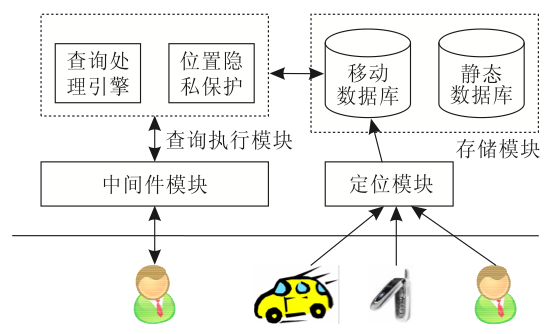
\includegraphics[bb=0 0 559 334, scale=0.45]{figure/fig_L10-2.png}
		\caption{LBS系统的架构}
		\label{fig:L10-2}
	\end{figure}

  通常,一个LBS服务提供商具备如下几方面特点\cite{L10}:高性能、可扩展性、高可靠性、实时性、移动性、开放性、安全性和互操作性。

	\subsubsection{基于空间信息网络的分布式思想的平台架构}
  刘丹、彭黎辉利用基于空间信息网络(spatial information grid, SIG)的分布式思想对空间位置服务平台的架构进行了模型设计和实现,完成了地图数据和定位查询的分布式存储和检索\cite{L08}。该平台服务满足开放位置服务(Open Location Service, 简称OpneLS)规范,利用XML进行信息编码,通过HTTP进行数据传输。同时,还针对定位信息的更新和传递提出了一种新的基于Push的主动通知机制,提供与各种定位接口的数据转换和消息处理能力,高效地实现了位置应用和服务平台之间地消息传递。

	\begin{figure}[htbp]
		\centering
		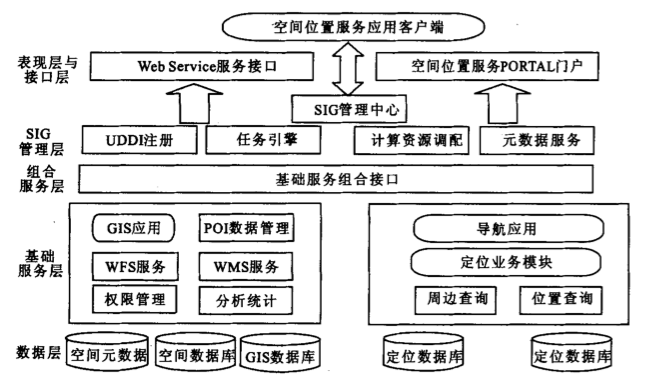
\includegraphics[bb=0 0 647 384, scale=0.45]{figure/fig_L08-4.png}
		\caption{SIG分布式架构}
		\label{fig:L08-4}
	\end{figure}

	LBS面向的空间数据量通常很大,涵盖的范围也不等,而SIG分布式架构网络化地设计和管理思想,可以有效地组织和管理这些数据,将各不同地域的数据托管在相应服务子站点服务器上,同时,这也很好的降低了用户集中访问同一台服务器造成的数据拥塞情况的发生。然而它也存在一定的缺点,分布式的平台架构在成本和管理力度上,则是一般中小企事业难以承受的。

	\subsubsection{基于J2EE的平台架构}
  蒋郁、刘伟平等人在LBS平台的设计过程中参考J2EE结构模型,并采用了组件式的设计方式,将整个平台划分成综合管理模块、GIS地理信息处理模块、接口层处理模块三大部分。此外,每个功能子模块独立封装,并对外提供统一规定的接口函数以供调用\cite{L06}。其中,综合处理模块作为整个平台的核心,负责将移动终端和业务服务联系起来,使移动用户获得所需的业务服务,其次还有用户认证、注册、计费等管理;GIS地理信息处理模块负责提供管理和处理大容量地图数据;LBS接口层处理模块负责和外部网络进行通信,使平台能在多种网络情况下运行,并且获得定位信息。基于J2EE开发模式的LBS平台系统工作流程如图\ref{fig:L06-2}所示:

	\begin{figure}[htbp]
		\centering
		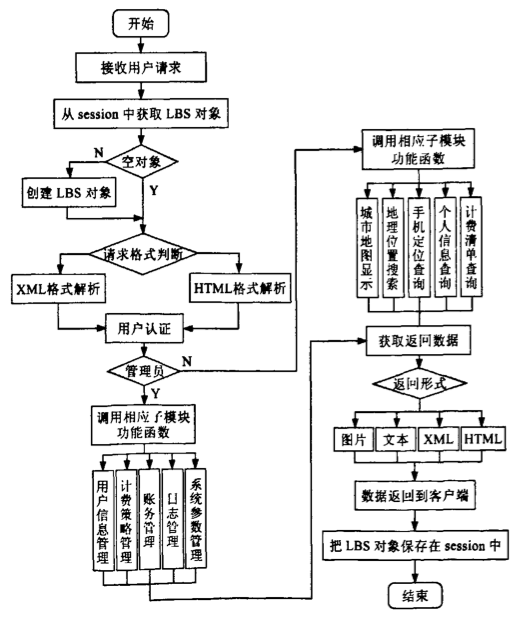
\includegraphics[bb=0 0 516 621, scale=0.45]{figure/fig_L06-2.png}
		\caption{基于J2EE开发模式的LBS平台系统工作的数据流程}
		\label{fig:L06-2}
	\end{figure}

  基于J2EE结构模型而设计实现的LBS系统平台,由于采用跨平台编程语言Java实现,所以具有良好的可移植性、可扩展性和平台无关性。另外,采用XML作为数据的统一格式,为不同平台的开发提供了方便。Jae-Chul Kim等人提出的平台架构也采用了XML作为数据的描述语言\cite{L13}。采用Web服务架构的平台,可以使得客户端的开发不受限于编程语言。

	\subsubsection{基于SOA的面向服务LBS}
  邹永贵、王剑提出了将SOA(Service-oriented Architecture,面向服务架构)架构运用于LBS,结合中间件技术,运用开放的Web服务技术,较好地解决了用户访问方式多样、异构兼容性不足和开发维护不易等问题\cite{L09}。

	\begin{figure}[htbp]
		\centering
		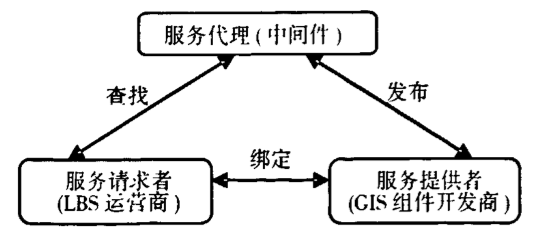
\includegraphics[bb=0 0 544 244, scale=0.45]{figure/fig_L09-2-1.png}
		\caption{面向服务的LBS定位服务平台构建模型}
		\label{fig:L09-2-1}
	\end{figure}

	\begin{figure}[htbp]
		\centering
		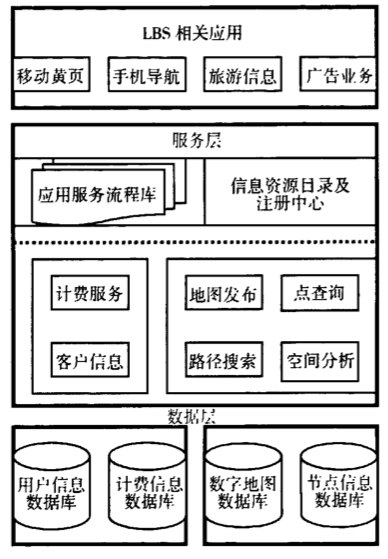
\includegraphics[bb=0 0 388 559, scale=0.45]{figure/fig_L09-2-2.png}
		\caption{面向服务的LBS定位服务平台架构}
		\label{fig:L09-2-2}
	\end{figure}

	从系统开发的角度来说,由于构建的LBS平台引入了中间件,所以只要求运营开发商具备一般的系统开发能力即可,开发的技术难度较小。GIS平台及相关硬件不需要运营商承担,因此开发成本也大为降低。同时,由于使用了基于XML的统一接口,所以开发灵活度也很高。

	而从系统应用角度来说,运营商只需要关注上层应用的日常运行和运营服务平台及流程服务器的更新,而底层包含核心应用模块的中间件则是由各GIS开发商负责的。这很大程度地降低了运营商对系统的运营成本和维护力度。

	\subsubsection{其它架构和方法}
  除了以上几种主流的架构方法外,还存在一些研究人员提出的其它架构方法,包括Aaron等人提出的一个开放式的基于SAGESS(Spatial Application Generic Environment System Standards,空间应用通用环境管理体系标准)的架构,以通过无线网络向用户提供富文本智能地图\cite{L05};W. Ait Cheik Bihi等人提出的TransportML\cite{L03};Rui Cheng等人提出的采用GIS、LBS、J2ME技术和地理数据结合而产生的平台:iZone,该平台可以为智能手机提供许多社交网络相关的服务\cite{L11};Paul J. Kuhn提出的LCBS\cite{L04}。


	\subsection{数据更新和获取}
  LBS的另一个重要服务便是信息服务,信息服务有源数据、信息有效期限、受众目标、位置依赖情况四个影响因素\cite{D06},改变其中任何一个都将影响到服务质量的好坏。用户在使用提供LBS技术的应用时,可能需要偶尔地,甚至随时随地地更新自己所在位置的相关信息,比如路径导航服务,就需要实时地对用户的当前位置进行更新,并同时获取道路交通情况信息。而如何处理数据的更新和获取,以及如何提升数据抓取的效率问题上,正是时下研究的热点之一。
   
  在数据更新方面,Suleiman Almasri等人提出的基于区域的更新机制\cite{L12},将一张大的地图划分成若干小的区域,用户只需下载自己所在位置的区域地图,所以,该更新机制可以大量减少信息传输量,很好的控制了网络带宽的使用,不仅提升了LBS性能,也最大限度地降低了用户设备的内存使用和功率消耗情况。

  在获取数据方面,各种数据挖掘技术已被广泛应用于从庞大且复杂的数据中获取到有价值的信息之中\cite{D09}。由于LBS系统的终端设备处理能力较低,显示屏幕较小,再加上无线数据网络带宽不足,因此无法浏览整个Web页面。采用信息抽取技术可以将用户感兴趣的信息提取出来,再发送给用户终端,有效地解决上述问题\cite{D11}。信息的过滤抽取可以减少冗余信息的传输,从而减少带宽的使用,提升数据的传输效率。随着移动技术地飞速发展,海量数据的传输也将变得容易,然而,对于用户来说,获取到真正有用的数据才是最重要的。通过信息抽取技术,所有发送到用户终端的数据都将根据用户所在位置和位置相关的信息进行过滤。用户还可以自定义信息的类别,以保证获取到自己更需要的信息,而不仅仅是位置相关的导航信息,而这也将为用户旅行在外提供更多方便和乐趣\cite{D10},此外,还可以为用户提供自动新闻概要服务\cite{D02}。

	\begin{figure}[htbp]
		\centering
		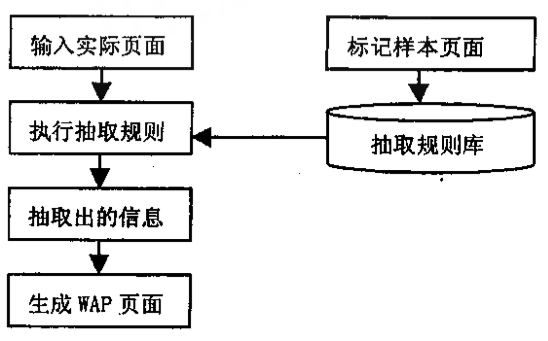
\includegraphics[bb=0 0 548 341, scale=0.45]{figure/fig_D11-2.png}
		\caption{基于LBS的信息抽取体系结构}
		\label{fig:D11-2-1}
	\end{figure}

  也因此,有人提出基于上下文和位置的服务(context and location bsed service)\cite{D05},为用户提供更个性化的自定义设置,从而提供更好的用户搜索查询体验(包括同一相关集群下的分组服务\cite{D05}、基于位置的抓取和推送服务\cite{D04})。

  Kahkashan Tabassum等人研究讨论了不同情形下,分布式处理位置相关的连续查询请求中遇到的各种挑战\cite{D08},并介绍了可以采用缓存和预加载技术,加大数据和查询结果的重用度,从而加快访问和响应的速度。另外,Shiow yang Wu等人提出的数据管理方法\cite{D06},也恰当地采用了缓存技术来提升LBS的效率。

  上述都是室外基于位置获取信息的一些技术方法,而现如今,室内的定位技术(如Kuofong Kao等人提出的通过将接入点作为信号强度数据采集器来实现室内的基于位置的服务\cite{D03})也在不断地被研究和实现,以适应今后不断增加的精度需求。

	\subsection{用户隐私}
  由于位置信息本身就易受伪造攻击(forging attacks),所以必须使用额外的机制以验证其完整性\cite{P04}。与此同时,保护用户的位置隐私也显得非常必要。位置隐私分为两类\cite{P02}:(1)敏感位置隐私,即用户对于所处位置比较敏感,希望自己的位置不被暴露;(2)位置-ID隐私,即攻击者能结合其它信息,根据用户的位置推断出用户的ID,导致用户的查询内容被暴露,此时用户对位置信息并不敏感,对查询内容是敏感的。

  隐私保护技术需要在保护隐私的同时,兼顾对应用的价值以及计算开销。通常可以从隐私保护度、数据缺损和算法性能三方面对隐私保护技术进行度量\cite{P01}。目前,一些实际可行的隐私保护方法已经得到研究并采用,比如基于二项式混合的位置匿名法\cite{P03}、基于点对点的隐蔽算法\cite{P05}、连续请求下的位置匿名方法\cite{P02}以及位置匿名化技术\cite{P01}等。各种隐私方法都有各自的不同特点,在不同需求下得到的效果也不尽相同。当针对特定数据实现隐私保护且对计算开销要求比较高时,基于数据失真的隐私保护技术更加适合;当更关注于对隐私的保护甚至要求实现完美保护时,则应该考虑基于数据加密的隐私保护技术,但代价是较高的计算开销(在分布式环境下,还会增加通讯开销)\cite{P01}。


	\section{已有相关关键技术的研究分析}
	\subsection{游戏客户端开发平台}
  2007年,苹果公司推出一款结合相机、手机、个人数位助理、媒体播放器及无线通信装置的手持设备:iPhono,取得很大反响,随后又相继推出了iPhone 3G、iPhone 3GS、iPhone 4,以及目前最新的iPhone 4S。iPhone采用优化了的OS X系统:iOS,并采用ARM处理器,能够平滑流畅地运行大部分应用。无论是外观设计还是用户体验,iPhone都是值得称道的。

  iOS平台已经极大地改变了新一代移动游戏的前景,它的独特性、连接性、个人集成性,流行以及新颖的界面,吸引了无数开发者。iPhone独特的用户界面已经派生了一些全新类别的游戏。改变设备倾斜的角度可以控制倾斜类的游戏,例如Lima Sky开发的Doodle Jump和NimbleBit开发的Scoops;多点触摸的游戏(例如Igloo Games开发的Bed Bugs)可以使得用户专注于游戏,因为它迫使用户同时操作多个游戏对象;Smule开发的娱乐应用程序Ocarina和Leaf Trombone允许用户通过向iPhone的麦克风吹气来弹唱虚拟乐器\cite{B02}。

  另外,iPhone拥有强大的多媒体设备。高分辨率的显示屏,以快速的响应时间消除图像残影,即使是以60帧每秒运行的游戏也不会有卡屏的问题。它自带有优秀的音频处理器,通过硬件音频解码,CPU可以关注游戏逻辑处理,而不用忙于播放背景音乐。

  iPhone、iPad和iPod touch除了支持多点触摸输入、硬件加速的3D和2D图像,以及健壮的音频工具包之外,还带有很好的通信能力。
  
  前所未有的连接性是将iPhone和过去其它移动游戏平台区分开的另一个功能。面向iPhone(或iPad touch)的开发人员可以认为他们的游戏始终拥有一个数据连接。这意味着iPhone上的游戏可以使用Internet连接性——既可以是游戏本身的核心部分(多玩家游戏),也可以是增强离线游戏体验的一部分(高分榜),还可以和社交网络集成,例如Facebook和Twitter。例如Com2uS开发的Baseball Slugger可以让您在卧室、公园长凳上或公交车座上和世界上其他任何地方的玩家进行对战。

  即使设备没有和Internet连接上,开发人员还可以通过蓝牙来连接玩家。另外通过推送消息的功能,甚至在玩家没有玩游戏的时候也可以参与到游戏中。并不是为非实时多玩家交互设计的游戏,例如ngmoco:)开发的Rolando 2通过iPhone的连接能力向其他玩家发送异步的挑战。这种技术特别适合于在回合制的游戏、或对手发出挑战的时候、或玩家记录被刷新的时候通知玩家。\cite{B02}

  在一台设备中集合了所有这些技术,使得这个平台成为创建多玩家游戏的理想平台。

	\subsection{用户终端的定位}
  苹果公司为iOS平台的开发提供了开发工具包:iOS SDK,它采用Objective C语言,将许多底层处理进行封装,提供API供开发者使用。比如iOS SDK中含有一个CoreLocation框架库。使用CoreLocation框架,可以确定设备当前的经度和纬度,从而提供位置相关的设置和事件。该框架通过硬件设备获取附近的信号,从而定位用户的位置\cite{iOSLIB}。这大大降低了LBS应用开发者的负担,也推动了LBS技术的发展。

	\subsection{地图服务:Google Maps API}
  Google Maps的出现,把传统的GIS从高校、科研机构、政府部门和建筑设计等应用领域,推向了寻常百姓,有如当年互联网从高校或是科研机构走向大众的过程一般。电子地图、行车指南、本地搜索等功能为老百姓的生活提供了极大方便。

  Google Maps API是Google为开发者提供的Maps编程API。它允许开发者在不必建立自己的地图服务器的情况下,将Google Maps地图数据嵌入到网站之中,从而实现嵌入Google Maps的地图服务应用,并借助Google Maps的地图数据为用户提供位置服务。值得一提的是,Google Maps API最大的优势,在于它是一个开放的系统,即用户完全可自定义非常的内容,从功能的地图、控件、事件,到专业的地图坐标系、地图类型、周边搜索等,用户通过Google Maps API均可以自定义。

  Google在推出地图、卫星图之后,又推出了地形图,它可以让用户在Google Maps上看到地图的三维地形。这是一个非常有用的功能,新的地形模式主要侧重于地图的物理特性,如高山、峡谷、植被等。地形模式甚至可以包含非常小的山、山路,并且使用只有细小差别的明暗来让人们更好地从卫星图片上理解地理高度的变化。\cite{B01}

	\subsection{局域网多人游戏}
  苹果为iOS平台的开发提供了三种发送和接收数据的方式:Wi-Fi(802.11无线网络标准)、蓝牙(Bluetooth)和蜂窝数据网络,所有方式都要使用无线电频率\cite{B02}。

  iOS SDK提供CFNetwork框架,它是一个很好的对Berkeley套接字的Objective C包装器,通过CFNetwork能够更轻松地编写网络代码,而且能很好地和iOS SDK中的其它框架合作。CFNetwork还向开发人员提供了HTTP协议和FTP协议的实现,并且将套接字和运行循环集成在一起,使得处理各类TCP/IP网络事件变得简单。

  为了推进多玩家游戏的开发,苹果还在iOS SDK中加入了一个包含多个工具的GameKit框架,使得这种类型游戏的创建过程变得更简单。该框架具有两大功能:

	\begin{enumerate}
		\item 通过蓝牙连接的点对点网络。
		\item 支持两个玩家之间的语音聊天。
	\end{enumerate}

  设计多玩家游戏的一个最大挑战就是,确定需要在应用程序的不同实例之间通信的信息。频繁地发送所有数据,将会导致迅速占满设备的通信通道,并且将电池耗尽。因此,必须仔细挑选需要在peer之间共享的信息,以及哪些信息是可以忽略的。通常采用以下方法解决:

	\begin{enumerate}
		\item 定义一个新的消息类型。
		\item 当和这个消息有关的事件发生的时候,向对方发送一个这个新类型的消息。
		\item 确保正确地处理收到的这个类型的消息。
  \end{enumerate}

  除此之外,对于在线多玩家游戏的开发人员来说,慢速的通信是要面对的更为严重的问题之一,而且这个问题是无法避免的,只能通过编码来绕过该问题。


	\section{总结与展望}
  本文献综述通过搜集整理LBS相关技术的论文、期刊、书籍,详细阐述了当今国内外LBS相关技术的研究现状,包括LBS系统的架构、数据更新和获取、用户隐私等。同时,也对现在已有相关关键技术进行仔细分析,归纳总结出一些适合本项目——基于位置服务的口袋妖怪类游戏的技术,为后期的项目开发做出理论基础和实际可行性上的验证。

  随着移动通信和卫星定位技术的不断发展,LBS技术正越来越受到人们的关注,研究深度也不断增加,相信在未来几年内将有一个快速的发展。它将改善人们的生活,成为人们生活中必不可少的一部分。再加上移动智能手机市场的不断扩展,随时使用许多包括LBS技术在内的高端技术已经成为可能。休闲游戏已是现在人们居家旅行消遣的重要对象,而基于LBS技术的休闲游戏,正是目前市场所缺少的,也是非常需要的。

	% Import references datas
	\bibliography{references.bib}

	\end{CJK}
\end{document}
